\section{Theory} \label{tex:theory}
In this section, the theory used to develop the methods and obtain the result in this thesis will be discussed. First, neural networks (NNs) will be covered - both the simpler artificial NNs (ANNs) and more complex networks such as the convolutional NN (CNN) in both 2 (image) and 3 (videos) dimensions. Also methods for calculating the theoretical speed of a NN will be covered. This is followed by the theory behind tensors and different methods in tensor decomposition. There will be more focus on Tucker decomposition since it is the one used in this thesis, and how to choose the appropriate rank in the case of Tucker decomposition.
\begin{figure}[H]
    \centering
    \captionsetup{width=.95\linewidth}
    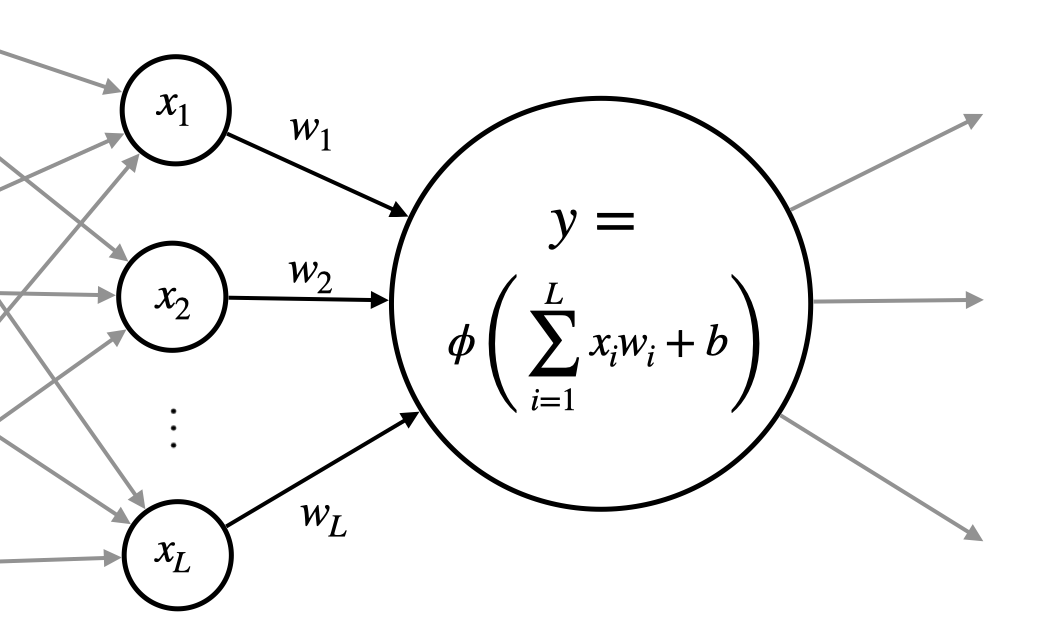
\includegraphics[width=.7\linewidth]{Pics/02_Theory/activation_illustration.png}
    \caption{Illustration of the flow of information through a neuron. Each edge (arrow) has a weight $w$ associated with it, and each neuron (circle) has an activation associated with it. The activations correspond to the information that is passed through the network, i.e. in this case the $L$ $x$s are used as inputs into the big neuron, where $y$ will be the resulting activation. $\phi$ is a non-linear transform called the activation function.}
    \label{fig:activation_illustration}
\end{figure}


\subsection{Neural Networks}\label{tex:theory_NN}
The NN is a very useful tool in non-linear classification and regression. It gets its name from what gave rise to the idea of it around half a century ago - the brain. Similar to the brain, a NN consists of a network of neurons that pass on information between each other. The way this is done is illustrated in \autoref{fig:activation_illustration}. Each neuron is, with a given input, associated with a value called its activation. This activation is based on the inputs to that very neuron, and is what is passed on from that neuron. The activation is calculated as the weighted sum of the activations of the inputs to that neuron plus a bias, all non-linearly transformed using an activation function $\phi$. Typical choices of $\phi$ are given in \autoref{fig:activation_functions}, while the typical activation of the last layer (the output) is the softmax-function, given by:
\begin{equation}
\text{Softmax:} \ \ \sigma: \R^K \rightarrow \R^K \qquad \sigma(\bs{x})_i = \frac{e^{x_i}}{\sum_{k=1}^K e^{x_k}} \quad \text{where} \ \bs{x} \in \R^K
\end{equation}
This is due to its ability to ensure a sum of 1 of all the outputs. In the end this value is the probability of the input belonging to each of the output classes. The predicted class is the one that has the highest probability.
\begin{figure}
    \centering
    \captionsetup{width=.95\linewidth}
    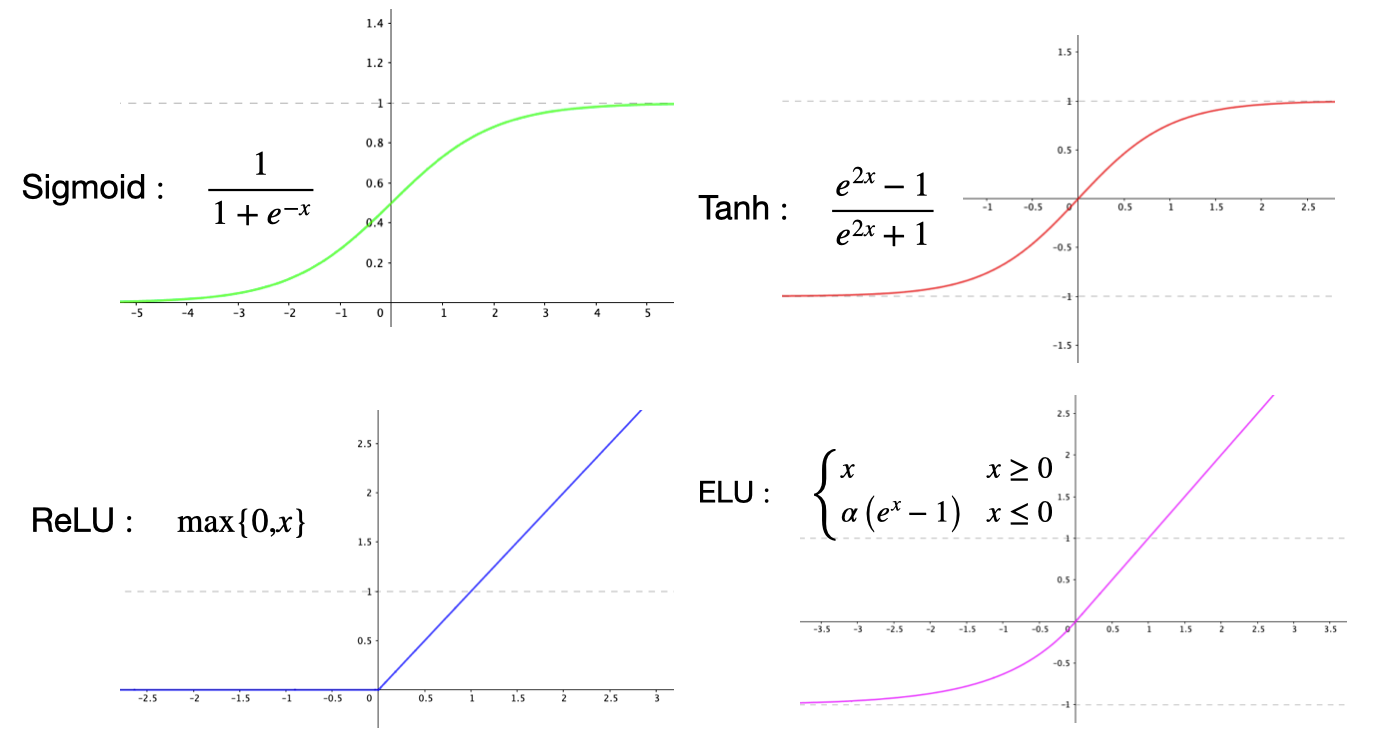
\includegraphics[width=.7\linewidth]{Pics/02_Theory/activation_functions.png}
    \caption{Typical activation functions used in NNs which are all non-linear transforms. The dotted grey lines represent the values of -1 and 1.}
    \label{fig:activation_functions}
\end{figure}

The size and layout of a NN is called the network architecture. The simplest type of NN architecture is the ANN. An example of a very simple ANN with only 2 input values for each observation, and binary output is given in \autoref{fig:very_simple_ANN}. This network has only a single hidden layer with $H$ neurons. 
\begin{figure}
    \centering
    \captionsetup{width=.95\linewidth}
    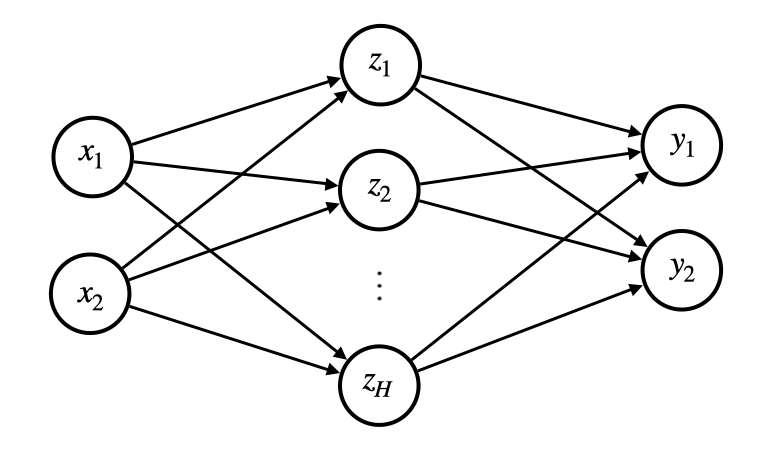
\includegraphics[width=.6\linewidth]{Pics/02_Theory/simple_ANN.png}
    \caption{Illustration of a very simple ANN with only 2 inputs $(x_1, x_2)$, 2 output $(y_1, y_2)$, and a single hidden layer with $H$ neurons $(z_1, z_2,\dots ,z_H)$.}
    \label{fig:very_simple_ANN}
\end{figure}

\subsubsection{Learning}
Learning a NN corresponds to finding the weights of the network that give the highest output accuracy - the best predictions. The method used to find the optimal weights is called back-propagation. This method simply sends inputs through the network and read the outputs. The output error is then propagated backwards through the network in order to adjust the weights accordingly. This is done repeatedly until convergence, normally dividing the training data into smaller batches and performing corrections using every batch. If the amount of data is limited, cross-validation is often used, which trains and validates on the same data. In cross-validation the data is split into a set of folds, and the network is trained on all the data except for one fold which is then used for validating the results.

To represent the error, a so-called loss function is used. Given an observation with input $\bs{x}$ and the corresponding true prediction $y$, we introduce the cost function given by:
\begin{equation}
    L(\Theta | \bs{x},y) = - \hat{p}(y) + \log\left(\sum_{k=0}^K e^{\hat{p}(k)}\right)
\end{equation}
Where $\Theta$ represents all the weights of the network, $K$ is the number of output classes, and $\hat{p}(k)$ is the predicted probability of the input belonging to class $k$. This function is also called the \textit{cross-entropy} loss function and is a the typical choice in classification problems. The cross-entropy loss function can be seen as a function of the weights of the network (here $\Theta$) because the weights are used to find the predictions $\hat{p}$. The gradient of this loss-function with respect to each of the weights in the network is used to update the weights accordingly by a gradient-descent step:
\begin{equation}
    \Theta_{new} = \Theta - \gamma \ \nabla L (\Theta)
\end{equation}
Where $\gamma$ is the learning rate that can be used to determine the speed of the learning, i.e. bigger values implies bigger jumps, while smaller values are used for fine-tuning. This derivative can be found either analytically, by applying the chain rule backwards through the network, or automatically using the \textit{autograd}-function in \textit{PyTorch}. In this thesis the \textit{autograd}-function will be used to find the derivatives, hence for the analytical derivations cf. \cite{elements_NN} or \cite{Zhang2016}.

\subsubsection{Architectures}
NNs are very flexible and can easily be adapted to fit every need. Not only can they be built off an arbitrary number of layers of different sizes, but also there are multiple different types of layers. Each layer finds progressively more complex features in the input data, hence more layers will be able to find more complex features. NNs can be both feed-forward (information flows forward) or recurrent (information flows backwards). The two types of layers that we will cover in this thesis are the dense layer and the convolutional layer respectively. Both have powerful properties and will be discussed further in the following.

\paragraph{The dense layer}
The dense layer is the basic building block of NNs, and ANNs are almost always built of these. A dense layer (also called fully-connected layer) is a layer in which each of neurons have a connection with all the neurons in the previous layer. Both the middle and output layers in the network illustrated in \autoref{fig:very_simple_ANN} are dense layers. In CNNs the dense layers are often used in the last part of the network to condense the information from the convolutional layers.

The dense layer is calculated as the non-linear transform of a matrix-vector product with the matrix consisting of the weights on the edges connecting the layer to the previous, and the vector being the input from the previous layer. This concept is illustrated in \autoref{fig:dense_layer_VM_prod}.
\begin{figure}
    \centering
    \captionsetup{width=.95\linewidth}
    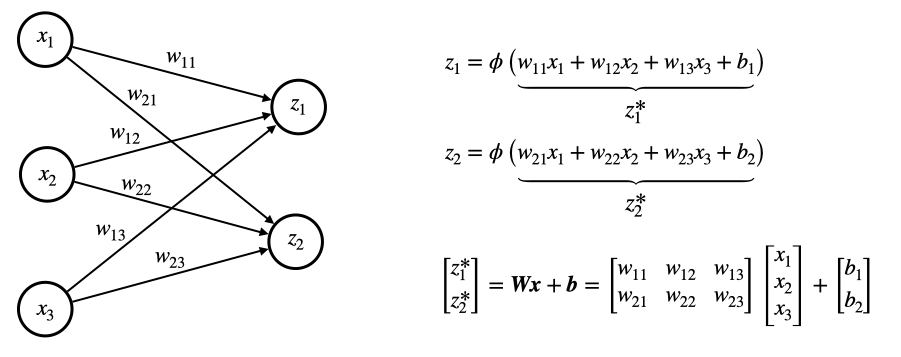
\includegraphics[width=\linewidth]{Pics/02_Theory/dense_layer_VM_prod.png}
    \caption{Illustration of the calculation of the dense layer. $x_i$ and $z_i$ are the $i$th activation of the two layers respectively. $w_{ji}$ is the weight corresponding to the connection between $x_i$ and $z_j$, and $b_i$ is the bias to be added to $z_i$. The dense layer is calculated as the non-linear transform of the bias plus the matrix-vector product between the weight matrix $\bs{W}$ and the input vector $\bs{x}$. $\phi$ is the activation function or non-linear transform.}
    \label{fig:dense_layer_VM_prod}
\end{figure}

\paragraph{The convolutional layer}
The convolutional layer has become a very powerful tool in image classification due to its ability to find features in images using the spatial information. In a convolutional layer the weights are arranged in a number of filters, each of which can be trained to look for specific features. For instance, a low-level filter can search for lines or curves in various directions, while higher-level filters look for e.g. faces, bodies, or wrinkles on clothes \cite{Yosinski2015}. The filters are placed in every position in the input image to calculate the activation at that position simply by multiplying the weights of the filter by the image and summing everything. The resulting activations will also be arranged as an image with high values corresponding to high activations.

Since color-images have multiple input channels (one red, one green, one blue), they are represented as order-3 tensors of size $H \times W \times S$, where $H$ is the image height in number of pixels, $W$ is the width of the image, and $S$ is the number of input channels. The convolution of an input image $\tensor{X}$ with this size into an output tensor $\tensor{Y}$ of size $H' \times W' \times T$ is given by:
\begin{equation}
    \tensor{Y}(h', w', t) =\sum_{i=1}^{D_H} \sum_{j=1}^{D_W} \sum_{s=1}^{S} \ \tensor{K}(i, j, s, t) \ \tensor{X}(h_i, w_j, s)
    \label{eq:2d_convolution_1}
\end{equation}
Where:
\begin{equation}
    h_i =  \left(h' - 1\right) \Delta_H + i - P_H \qquad w_j =  \left(w' - 1\right) \Delta_W + j - P_W
\end{equation}
In \eqref{eq:2d_convolution_1} $\tensor{K}$ is the 4-dimensional kernel of size $D_H \times D_W \times S \times T$ which corresponds to the $T$ different stacked filters of size $D_H \times D_W \times S$. $\Delta$ corresponds to the stride, i.e. how much the filters should move between each calculation (usually 1). $P$ corresponds to the padding which is how many 0s should be put on the edges of the image, and can be used to ensure the same input and output size in terms of the spatial dimensions. $(h_i, w_j)$ is the top left corner of the position in the input image and the three sums correspond to the application of the $t$th filter to that position. The application of a filter to an image with a single input channel is illustrated in \autoref{fig:convolution_illustration}.
\begin{figure}
    \centering
    \captionsetup{width=.95\linewidth}
    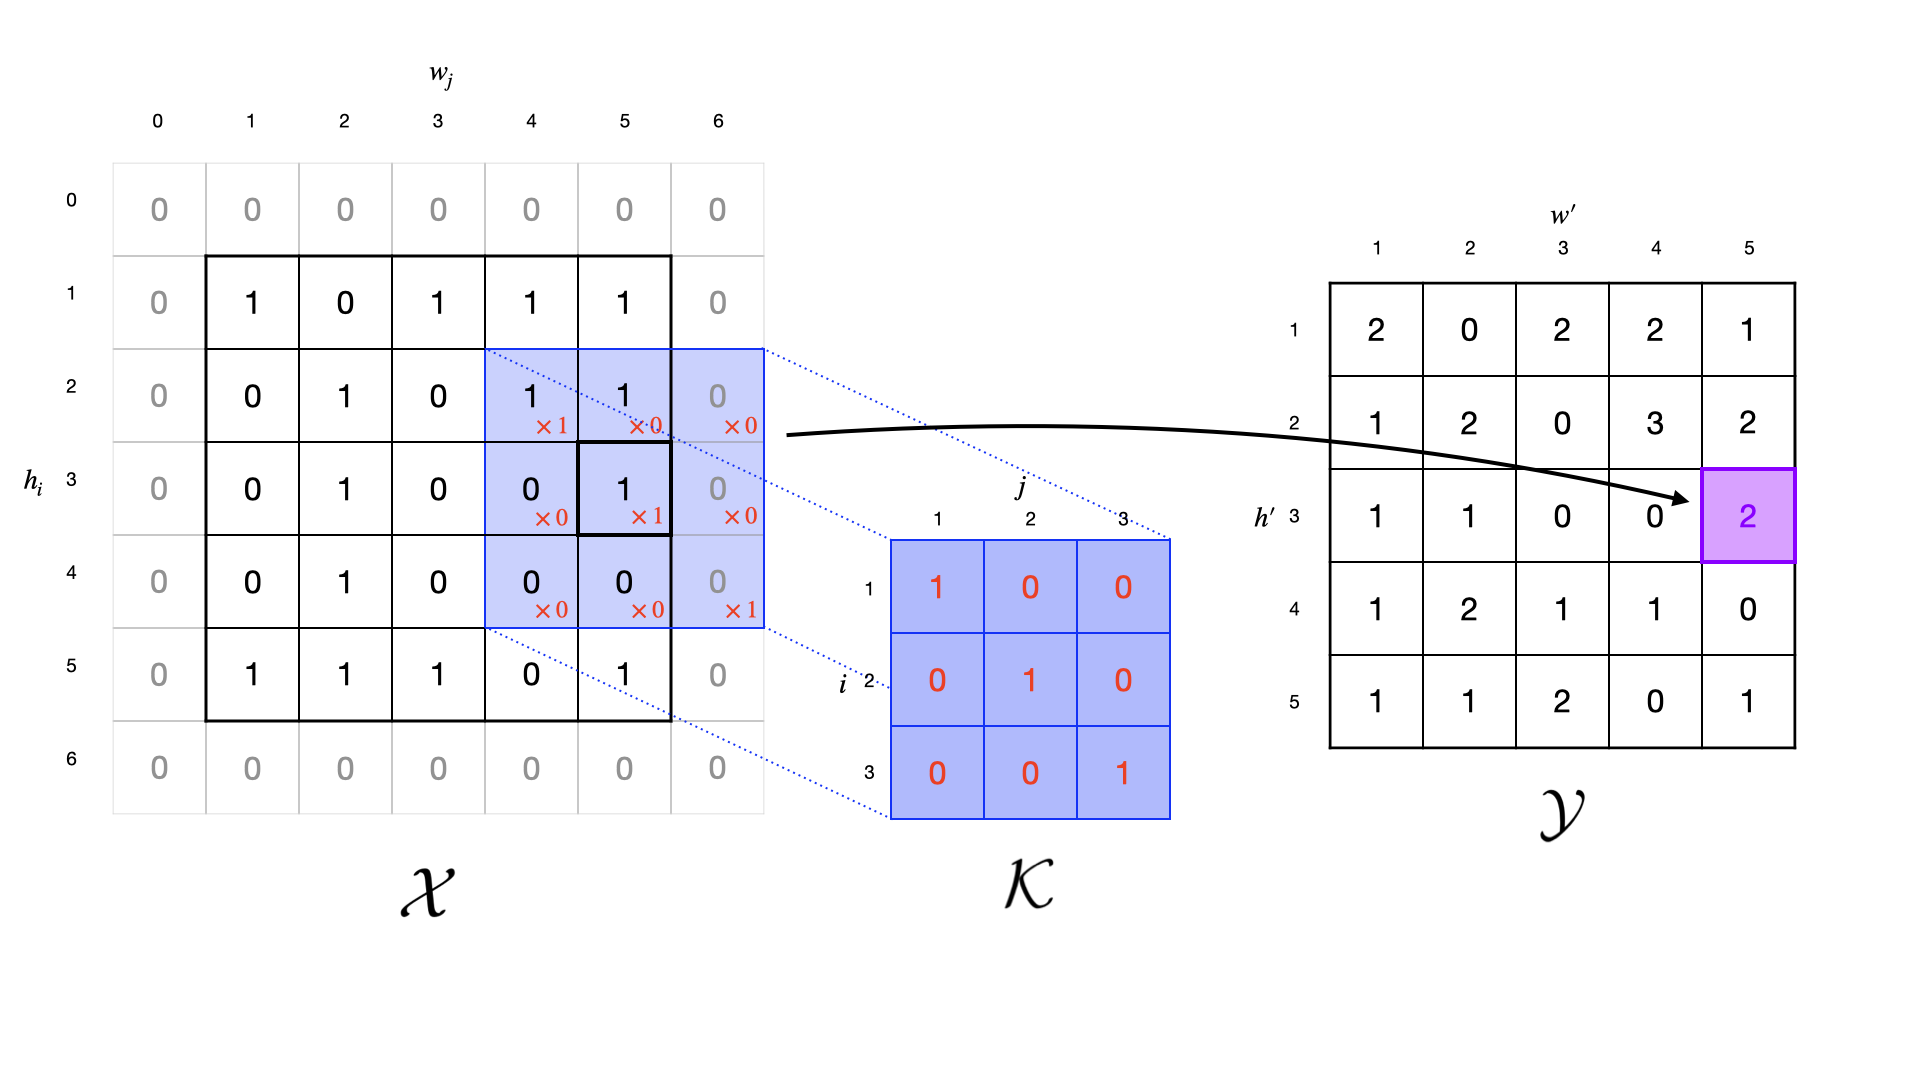
\includegraphics[width=\linewidth]{Pics/02_Theory/convolution_illustration.png}
    \caption{Illustration of a simple convolution of a picture with a single input channel. The calculation of the value $\tensor{Y}(3, 5, \cdot)$ is the one that is highlighted. The arrow signifies the sum of the result of applying the filter $\tensor{K}$ to the input image $\tensor{X}$. The input image will always be 1-indexed, hence the padding (grey 0s) is indexed appropriately. The very simple filter is trained to look for diagonal lines, hence the output will have a high activation if a diagonal line is present in $\tensor{X}$. If there are more input channels, the input image $\tensor{X}$ and the filter $\tensor{K}$ will both be 3-dimensional tensors.}
    \label{fig:convolution_illustration}
\end{figure}
The output size $H' \times W'$ is calculated by the formula:
\begin{align}
    H' &= \frac{H - D_H + 2\cdot P_H}{\Delta_H} + 1 \label{eq:out_dim_H}\\
    W' &= \frac{W - D_W + 2\cdot P_W}{\Delta_W} + 1 \label{eq:out_dim_W}
\end{align}
\subparagraph{The 3D convolution in videos}
There are multiple ways of doing convolutions for videos, that are simply a stack of images. One way is to do convolutions on every frame in a sequence and gathering the result - another way is to apply a 3-dimensional filter.\footnote{This filter will actually be 4-dimensional if there are multiple input dimensions} The 3-dimensional filter will not only look for features in the spatial dimensions, but also for temporal information, i.e. movement. The 3D convolution is very similar to the 2D case \eqref{eq:2d_convolution_1}, except for another sum and higher dimensions. The 3D convolution of an input video $\tensor{X}$ of size $F\times H \times W \times S$ ($F$ is the frames) into an output tensor $\tensor{Y}$ of size $F'\times H' \times W' \times T$ is given by:
\begin{equation}
    \tensor{Y}(f', h', w', t) = \sum_{i=1}^{D_F} \sum_{j=1}^{D_H} \sum_{l=1}^{D_W} \sum_{s=1}^{S} \ \tensor{K}(i, j, l, s, t) \ \tensor{X}(f_i, h_j, w_l, s)
\end{equation}
Where:
\begin{equation}
    f_i = \left(f' - 1\right) \Delta_F + i - P_F \qquad h_j =  \left(h' - 1\right) \Delta_H + j - P_H \qquad w_l =  \left(w' - 1\right) \Delta_W + l - P_W
\end{equation}
Now the convolutional kernel $\tensor{K}$ is 5-dimensional and have the size $D_F \times D_H \times D_W \times S \times T$, which is a stack of 4-dimensional filters. The output size $F'$ is calculated in the same way as \eqref{eq:out_dim_H} and \eqref{eq:out_dim_W} by:
\begin{equation}
    F' = \frac{F - D_F + 2\cdot P_F}{\Delta_F} + 1
    \label{eq:out_dim_F}
\end{equation}

%%%%%%%%%%%%%%%%%%%%%%%%%%%%%%%%%%%%%%%%%%%%%%%%%%%%%%%%%%%%%%%%%%%%%%%%%%%%%%%%%%%
%%%%%  Tensor Decomposition %%%%%%%%%%%%%%%%%%%%%%%%%%%%%%%%%%%%%%%%%%%%%%%%%%%%%%%
%%%%%%%%%%%%%%%%%%%%%%%%%%%%%%%%%%%%%%%%%%%%%%%%%%%%%%%%%%%%%%%%%%%%%%%%%%%%%%%%%%%

\subsection{Tensors and Tensor Decomposition}\label{tex:decomp_methods}
A tensor is a data array of an arbitrary number of dimensions, hence matrices are order-2 tensors, while vectors are order-1 tensors. Tensors are frequently used in many different fields that have to do with computer science\cite{Mørup2011}. Tensors have many great properties due to their many dimensions, but also quickly grow very large. Two central concepts used in calculations with tensors are matricization and the $n$-mode product, which will be discussed in \autoref{tex:tensor_operations}.

The concept of tensor decomposition or tensor factorisation concerns itself with exploiting the tendencies of the data in order to find a representation that is smaller and easier to work with. There are multiple representations or decompositions that will be discussed in detail later in this section. The Tucker method will be discussed in a bit more detail, due to its importance to the work done in the thesis. Since the python library \textit{TensorLy} has great implementations of the different algorithms, it will be used to calculate the decompositions throughout the thesis. The algorithms for estimating the decomposition are given in \autoref{app:DecompEstimation}.

\subsubsection{Basic tensor representation and operations} \label{tex:tensor_operations}
\paragraph{Tensor matricization}
It is often useful to reshape a tensor of order > 2 into a matrix. This is for instance in order to calculate the product of the tensor and a matrix. Tensors can be matricized with respect to one of its dimensions, i.e. using the $n$th dimension, the matricization of a tensor $\tensor{X}$ becomes:
\begin{equation}
    \tensor{X}^{I_1 \times I_2 \times \dots I_N} \xrightarrow[matricization]{} \bs{X}_{(n)}^{I_n \times I_1 \cdot I_2 \cdots I_{n-1} \cdot I_{n+1} \cdots I_N}
\end{equation}
Which means that the first dimension of the resulting matrix is equal to the $n$th dimension of $\tensor{X}$ while the second dimension will be equal to the product of the remaining dimensions. Going from a matrix to a tensor is called un-matricization or tensorizing and is given by:
\begin{equation}
      \bs{X}_{(n)}^{I_n \times I_1 \cdot I_2 \cdots I_{n-1} \cdot I_{n+1} \cdots I_N} \xrightarrow[un-matricization]{} \tensor{X}^{I_1 \times I_2 \times \dots I_N}
\end{equation}
Notice that the original (or desired) shape of $\tensor{X}$ must be know in order to tensorize a matrix. In XXX matricization of an order-3 matrix using each of the modes is illustrated.
\begin{figure}
    \centering
    \includegraphics{}
    \caption{Caption}
    \label{fig:my_label}
\end{figure}

\subsubsection{CP / Parafac}
CP (Candecomp) decomposition that also goes by the names of Parafac or canonical decomposition is the most basic representation. The CP decomposition represents the tensor as the sum of $R$ outer-vector products, where each dimension has a loading vector for each $R$. $R$ is the rank of the decomposition and obviously this allows for more specific details the higher $R$ gets. The CP decomposition of an order-3 tensor $\tensor{X}$ of size $n_1\times n_2 \times n_3$ is given by:
\begin{equation}
    \tensor{X} \approx \sum_{d=1}^R \bs{a}_d \circ \bs{b}_d \circ \bs{c}_d
\end{equation}
Or element-wise:
\begin{equation}
    \tensor{X}(i, j, l) \approx \sum_{d=1}^R \bs{a}_d(i) \cdot \bs{b}_d(j) \cdot \bs{c}_d(l)
\end{equation}
Where $\boldsymbol{a}_i$, $\boldsymbol{b}_i$, and $\boldsymbol{c}_i$ are the $i$th loading vectors of each dimension respectively. If each of these loading vectors are concatenated to form loading matrices, the decomposition can also be written in the following way using a diagonal or identity tensor $\tensor{D}$ and $n$-mode products:
\begin{equation}
    \tensor{X}^{n_1 \times n_2 \times n_3} \approx \tensor{D}^{R\times R\times R} \times_1 \bs{A}^{n_1 \times R} \times_2 \bs{B}^{n_2 \times R} \times_3 \bs{C}^{n_3 \times R}
    \label{eq:CP_matrix_rep}
\end{equation}
$\tensor{D}$ is also called the core tensor. For the loading matrices we have that:
\begin{equation}
    \bs{A} = \begin{bmatrix} | & | & & |\\ \bs{a}_1 & \bs{a}_2 & \dots & \bs{a}_R \\ | & | & & | \end{bmatrix} \qquad \bs{B} = \begin{bmatrix} | & | & & |\\ \bs{b}_1 & \bs{b}_2 & \dots & \bs{b}_R \\ | & | & & | \end{bmatrix} \qquad \bs{C} = \begin{bmatrix} | & | & & |\\ \bs{c}_1 & \bs{c}_2 & \dots & \bs{c}_R \\ | & | & & | \end{bmatrix}
\end{equation}
The CP decomposition is illustrated in \autoref{fig:CP_decomp_illustration}.
\begin{figure}
    \centering
    \captionsetup{width=.95\linewidth}
    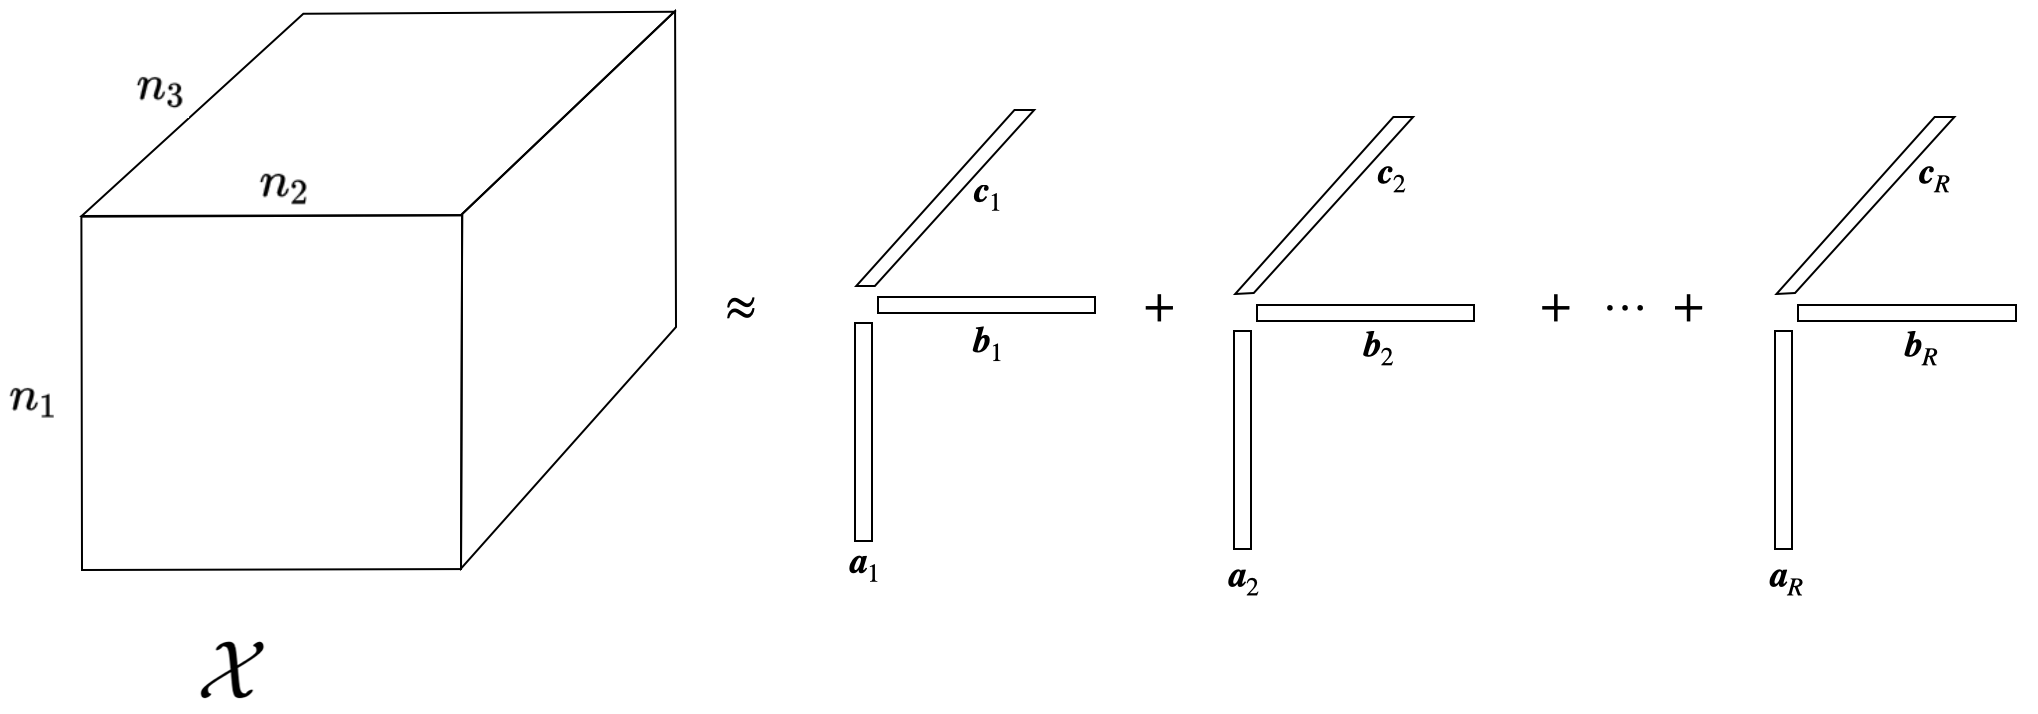
\includegraphics[width=\linewidth]{Pics/02_Theory/CP_decomp_illustration.png}
    \caption{The tensor $\tensor{X}$ is decomposed using the CP decomposition. The CP decomposition approximation is the sum of a sequence of $R$ outer-vector products, with $R$ being the rank of the decomposition. The vectors have length corresponding to the length of the dimension in $\tensor{X}$, e.g. all the $\bs{a}$-vectors have length $n_1$.}
    \label{fig:CP_decomp_illustration}
\end{figure}

Due to the nature of the CP decomposition only the $i$th loading of each loading vector can interact with each other, making the CP decomposition rather restricted. However the restriction of this representation implies a unique optimal solution of the CP decomposition, which desirable. The method is good at resolving different additive physical profiles, e.g. if addition of multiple chemicals to a solution have different effects on a response variable, these can be resolved. CP decomposition however fails when different dimensions are correlated, due to strong cancellation effects between the various components of the representation, making it slow to converge and hard to interpret \cite{Mørup2011}.

\subsubsection{Tucker}
Tucker decomposition is the less restricted version of the CP decomposition - or actually CP decomposition is a special case of Tucker. In Tucker decomposition loadings can interact with each other even crisscrossing, which gives this representation a good deal of freedom. This is achieved allowing the core-tensor $\tensor{D}$ ($\tensor{G}$ for Tucker) to be non-diagonal, hence we also get to choose special ranks for each dimension. Thus the Tucker decomposition is a sum of outer-vector products scaled by the core element. Based on the matrix-representation of the CP decomposition \eqref{eq:CP_matrix_rep}, the Tucker decomposition of an order-3 tensor $\tensor{X}$ of size $n_1 \times n_2 \times n_3$ is given as:
\begin{equation}
    \tensor{X}^{n_1 \times n_2 \times n_3} \approx \tensor{G}^{R_A \times R_B \times R_C} \times_1 \bs{A}^{n_1 \times R_A} \times_2 \bs{B}^{n_2 \times R_B} \times_3 \bs{C}^{n_3 \times R_C}
\end{equation}
Where $\bs{A}$, $\bs{B}$, and $\bs{C}$ are the loading matrices of each of the dimensions and $R_A$, $R_B$, and $R_C$ are the ranks of the decomposition in each of the dimensions. $\tensor{G}$ is the core tensor that we in the Tucker case allow to be non-diagonal. We can also write the Tucker representation element-wise:
\begin{equation}
    \tensor{X}(x_1,x_2,x_3) \approx \sum_{r_A=1}^{R_A} \sum_{r_B=1}^{R_B} \sum_{r_C=1}^{R_C} \tensor{G}(r_A, r_B, r_C) \cdot \bs{A}(x_1, r_A) \cdot \bs{B}(x_2, r_B) \cdot \bs{C}(x_3, r_C)
\end{equation}
The concept of Tucker decomposition is shown in \autoref{fig:tucker_decomp_illustration}. 
\begin{figure}
    \centering
    \captionsetup{width=.95\linewidth}
    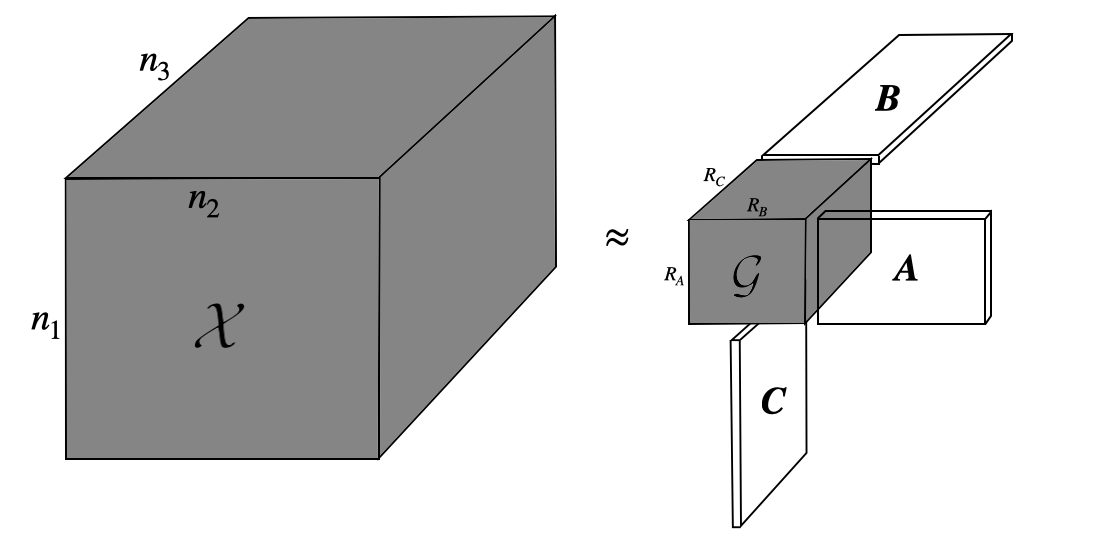
\includegraphics[width=.7\linewidth]{Pics/02_Theory/Tucker_decomp_illustration.png}
    \caption{The tensor $\tensor{X}$ is decomposed using Tucker-3 decomposition, which means that all 3 dimensions will be decomposed. The Tucker decomposition is a sequence of $n$-mode products between the core tensor $\tensor{G}$ and the three loading matrices $\bs{A}$, $\bs{B}$, and $\bs{C}$. The size of $\tensor{G}$ is equal to the ranks of the decomposition, i.e. $R_A \times R_B \times R_C$. The length of the first dimension of the loading matrices correspond to the length of the given dimension, e.g. for $\bs{A}$ it is $n_1$}
    \label{fig:tucker_decomp_illustration}
\end{figure}
The different rank along each of the dimensions, makes the user able to choose how many different features the algorithm should find along each dimensions. The flexibility of the Tucker decomposition makes it useful for many applications, one of them being the data compression task. The flexibility however also comes at a cost; the representation does not yield unique optimal solutions, and the results harder to interpret than for CP decomposition.

Rank selection for the Tucker decomposition is either choosing appropriate ranks for the problem, or to find the minimal set of ranks $(R_A, R_B, R_C)$ that ensure that:
\begin{equation}
    \tensor{X} = \sum_{r_A=1}^{R_A} \sum_{r_B=1}^{R_B}
 \sum_{r_B=1}^{R_B} \tensor{G}(r_A, r_B, r_C) \cdot \bs{a}_{r_A} \circ \bs{b}_{r_B} \circ \bs{c}_{r_C}
 \end{equation}
I.e. the approximation being equal to the actual tensor. Here $\bs{a}_i$, $\bs{b}_i$, and $\bs{c}_i$ are the $i$th column of the loading matrices respectively. Finding the optimal ranks is a challenging problem, which have been solved in different ways. Due to the challenge of the problem, this thesis will make use of the analytical solution to variational Bayesian matrix factorization (VBMF) by inspiration from Kim et. al \cite{Kim2016}. This approach is chosen because it is a good and easily reproducible heuristic, even though it is sub-optimal. VBMF will be discussed in the following.

\paragraph{Variational Bayesian Matrix Factorization} \label{tex:VBMF}
The global analytical solution to the VBMF have been derived by Nakajima et. al in 2013 \cite{Nakajima2013}, and can be used as a method for rank selection for the Tucker model\footnote{Also applicable to CP-decomposition, since it is a special case of Tucker decomposition}. The authors use a probabilistic model to find the optimal low-rank factorization of a matrix, automatically taking care of the noise. Given an matrix $\bs{V}$ of size $L\times M$ that is assumed to be the sum of a target matrix and an error matrix:
\begin{equation}
    \bs{V}^{L\times M} = \bs{U}^{L\times M} + \bs{E}^{L\times M}
\end{equation}
The goal is to find matrices $\bs{A}$ and $\bs{B}$ such that:
\begin{equation}
    \bs{U} = \bs{B}\bs{A}^{\top}
\end{equation}
This is achieved by considering a probabilistic model of $\bs{V}$ given prior variances, and use this model to compute the posterior distributions of $\bs{V}$, $\bs{A}$, and $\bs{B}$. Doing this is generally a non-convex problem why the analytical solution is key. This however does only work for matrices, hence tensors of order $> 2$ need to be converted into matrices using matricization discussed in \autoref{tex:tensor_operations}. Matricization using the $i$th dimension gives the estimated rank of that same dimension of the tensor. It should be noted that this method only works when the $L < M$, since we need to have $\frac{L}{M} < 1$ to satisfy the nature of the probabilistic distribution.

\subsubsection{Block-Term Decomposition}
Block-Term Decomposition (BTD) is simply a sum of Tucker terms, i.e. given an order-3 tensor $\tensor{X}$ and a rank $R$ the BTD of $\tensor{X}$ is given by:
\begin{equation}
    \tensor{X} = \sum_{r=1}^R \tensor{G}_r \times_1 \bs{A}_r \times_2 \bs{B}_r \times_3 \bs{C}_r
\end{equation}
Where we now have $R$ sets of a core and loading matrices instead of a single one of each, which also means that the ranks of the individual Tucker terms can differ to comply with various needs.

\subsubsection{Tensor-Train decomposition}
Tensor-Train (TT) decomposition that also goes by the name "matrix product state decomposition", was developed by Oseledets in 2011, as a simple and non-recursive tensor decomposition representation.\cite{Oseledets2011} TT-decomposition does not make use of a core tensor, but allows for all the loadings arrays to be order-3 tensors. Given an order-$d$ tensor $\tensor{X}$ of size $n_1\times n_2 \times \dots \times n_d$, we will have a sequence of ranks $r_0, r_1, \dots, r_d$, with boundary conditions $r_0=r_d=1$. The TT-decomposition of $\tensor{X}$ is given by:
\begin{equation}
    \tensor{X}(i_1, i_2, \dots, i_d) \approx \tensor{G}_1[i_1] \tensor{G}_2[i_2] \cdots \tensor{G}_d[i_d]
\end{equation}
Where $\tensor{G}_i$ is the $i$th loading tensor of size $r_{i-1}\times n_1\times r_i$, and $\tensor{G}_i[j]$ is the $j$th lateral slice of $\tensor{G}$, which makes it a matrix of size $r_{i-1}\times r_i$. The calculation of a single value at position $(i_1, i_2, \dots, i_d)$ is illustrated in \autoref{fig:TT_decomp_illustration}.
\begin{figure}
    \centering
    \captionsetup{width=.95\linewidth}
    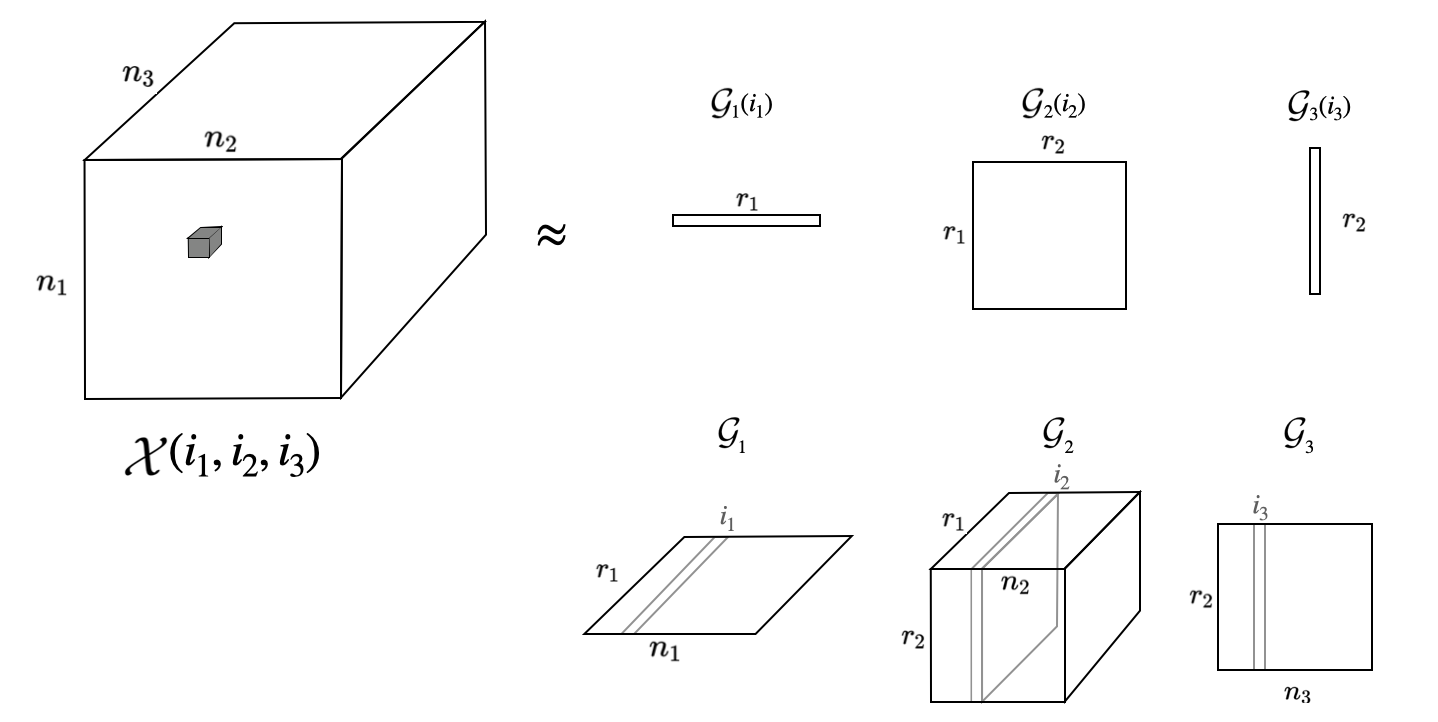
\includegraphics[width=.9\linewidth]{Pics/02_Theory/TT_decomp_illustration.png}
    \caption{The approximation of a single value of the target tensor using the TT-decomposition. The value is the result of a vector-matrix-vector product between $\tensor{G}_1(i_1)$, $\tensor{G}_2(i_2)$, and $\tensor{G}_3(i_4)$ that are slices of the loading tensors $\tensor{G}$. The bottom row shows how the vectors and the matrix are taken out of the $\tensor{G}$s using the given indices $i_1$, $i_2$, and $i_3$.}
    \label{fig:TT_decomp_illustration}
\end{figure}

The TT-decomposition is not prone to the curse of dimensionality, it is stable, and has asymptotically the same number of parameters as CP-decomposition. Oseledets have in \cite{Oseledets2011} also derived efficient versions of basic tensor operations in the TT-format.